
\resetcounters

\bibliographystyle{asp2010}

\markboth{Williams and Bridger}{Spectral Line Selection in the ALMA Observing Tool}

\title{Spectral Line Selection in the ALMA Observing Tool}
\author{Stewart~Williams and Alan~Bridger
\affil{UK Astronomy Technology Centre, Royal Observatory Edinburgh, Blackford Hill, Edinburgh, United Kingdom, EH9 3HJ}}

\aindex{Williams, S.}
\aindex{Bridger, A.}

\begin{abstract}
The Atacama Large Millimetre / submillimetre Array (ALMA) is the world's most powerful ground-based telescope, offering views of the mm/submm universe with unparalleled spatial and spectral resolution. With the high level of flexibility offered by ALMA, proposals making full use of its capabilities are complex and it would be easy for an inexperienced radio astronomer to request an invalid instrument configuration. In this paper we describe the hardware-aware filters and real-time filtering techniques used by the ALMA Observing Tool (OT) that lets astronomers efficiently identify their primary target lines and `lines of opportunity', all the while preventing the user from constructing invalid proposals.
\end{abstract}

\section{Introduction}
\label{sec:introduction}
The Atacama Large Millimetre/submillimetre Array (ALMA) is the world's most powerful ground-based observatory operating at mm/submm wavelengths, and the majority of ALMA observations are expected to be highly-targeted measurements of spectral emission lines. The details of these observations, including the desired hardware configuration, are specified using the ALMA Observing Tool (OT), a software tool used by astronomers to construct ALMA proposals \citep{bridger_2004}.

In order to accurately target spectral lines, astronomers consult a reliable reference catalogue of transition frequencies. To facilitate this process and provide a consistent data source, Splatalogue \citep{splatalogue} provides ALMA with access to its catalogue of rest frequencies for over six million transitions, accessible via the Simple Line Access Protocol \citep[SLAP;][]{SLAP}. When online, the OT can use SLAP to remotely query the full Splatalogue database, and so any of the millions of entries may be specified as target transitions of an observing proposal.

However, the OT is formally required to allow proposal preparation when network access is not available. To enable line selection while offline, a small database containing a subset of the complete Splatalogue collection is packaged with the OT. This offline database comprises around 21,000 of the most commonly observed and strongest lines expected to be seen with ALMA. In practical terms, it is expected to contain the vast majority of lines required by the community, and so only infrequently should it be necessary to resort to an online search of the full Splatalogue database. 

The provision of a local database has greatly influenced the design of the spectral line selector (SLS), the tool used within the OT to select spectral lines. This paper describes the SLS functionality enabled through the use of a small local data source. In \S\ref{sec:real-time queries}  we describe the real-time queries and user interface improvements that result, while in \S\ref{sec:hardware filters} we describe the filters that prevent the construction of unworkable proposals.

\section{Filter Pipeline and Real-time Queries}
\label{sec:real-time queries}
The database packaged with the OT is comprehensive enough for the preparation of most proposals, yet small enough to fit in memory. With the database residing in memory, queries can be executed and results found extremely quickly. Matches are returned almost instantaneously, as opposed to the several second latency experienced when querying a remote database. 

To take advantage of these low-latency queries, the line selector has been designed around a filter pipeline, to which user filters and automatic filters can be inserted, tweaked, and removed in response to user actions (Figure~\ref{fig:pipeline}). This reverses the usual search perspective, where the user begins with an empty pool and query results are made available for selection, to a view where the user begins with the complete database (Figure~\ref{fig:Wscreenshot}), and their subsequent interactions progressively filter transitions out. 

Details of the target objects, including their radial velocity, are input into the OT when specifying a new proposal. On the addition or activation of any frequency filter, the SLS can use these data make the appropriate Doppler-correction. This ensures the sky frequency is always considered, and not the rest frequency as recorded in Splatalogue.

\begin{figure}
	\includegraphics[width=0.873\textwidth]{part10/Williams_O32/O32_f1a.eps}
	\includegraphics[width=1.0\textwidth]{part10/Williams_O32/O32_f1b.eps}
	\caption{Conceptual diagram of filter pipeline with no lines selected (upper) and with lines selected and automatic filters engaged (lower). Automatic filters and user-configurable filters are depicted in green and blue respectively.}
	\label{fig:pipeline}
\end{figure}

\begin{figure}
	\includegraphics[width=\textwidth]{part10/Williams_O32/O32_f2.eps}
	\caption{Screenshot of the spectral line selector on first launch.}
	\label{fig:Wscreenshot}
\end{figure}

The spectral line selector re-filters the complete dataset on each key press and widget event, thus giving the user immediate feedback on changes to filter constraints. With queries executed and results found in real-time, it is easy to experiment and incrementally build a query until the target transition is identified. Additionally, by building and executing a query piece-by-piece, it becomes easy to identify which addition led to an overly-restrictive filter, letting the user quickly revert to the last-good state.

Dynamic filtering of lines from an initially full pool helps the user experience in several ways. An immediate benefit of initially presenting all entries to the user (Figure~\ref{fig:Wscreenshot}) is to let the user orient themselves with the Splatalogue line description format, which may differ to how the astronomer is accustomed to describing lines (eg., `CO 1-0' vs. `CO v=0 J=1-0'). Transitions are also identified by formulae and quantum numbers that may contain subscripts, subscripts and non-ASCII characters. Filtering on each user event quickly brings the target line into view after minimum input, rendering further entry of the less accessible characters unnecessary.

\section{Filtering Based on Hardware Constraints}
\label{sec:hardware filters}
ALMA is a flexible instrument, but this flexibility could easily make the instrument difficult to use for an astronomer unfamiliar with tuneable heterodyne receivers. Most complexity arises when constructing a proposal to observe multiple spectral lines simultaneously. In this situation, the tuning required by one line affects which other transitions can be simultaneously observed; it would be easy for an astronomer unaware of the implications of tuneable receiver front-ends and back-ends to request an invalid configuration. To help prevent the construction of unworkable proposals, the spectral line selector has additional filters that are aware of the various ALMA hardware limitations. 

Firstly, an 'Available Receivers' filter is inserted into the pipeline  (Figure~\ref{fig:pipeline}: `Available Receivers Filter'). ALMA is still under construction, and not all receivers have been commissioned. To limit the selection of lines to available receiver bands, the available receivers filters out those transitions outside the range of an available receiver. 

Secondly, the pipeline has filters that are aware of the tuneable aspects of ALMA hardware (Figure~\ref{fig:pipeline}: `Sideband' and `Baseband' filters). Together, these filters work by ensuring the lines available for selection can always be simultaneously observed with those transitions already present in the proposal. Unlike user filters, these automatic filters are not user-configurable, and are automatically created on the addition of each line to the proposal. 

Figure \ref{fig:filter construction} illustrates the construction and operation of a typical tuning-aware filter. For any given line, the hardware could be tuned so that a range of companion frequencies could be detected while still covering that transition (Figure~\ref{fig:filter union}). Conceptually, these tuning possibilities are best visualised as a set of windows overlaid on each line selected in the proposal (Figure~\ref{fig:sidebands}). Transitions lying outside these windows cannot be co-observed, and are thus removed. By determining the intersecting frequency range of these filters, we determine the range of frequencies that may be simultaneously observed, and hence which transitions should be made available for selection. With the filters removing all transitions outside the range of possible tunings, it becomes impossible for the user to select a combination of lines that cannot be simultaneously observed.

As a final consideration, with lines added to a proposal but no user filters active, the SLS displays all lines potentially observable given the current hardware configuration. Astronomers can use this facility to find `lines of opportunity`: additional, secondary transitions that were initially unconsidered but may be of scientific interest.

\begin{figure}
\centering
\begin{subfigure}[b]{0.5\textwidth}
	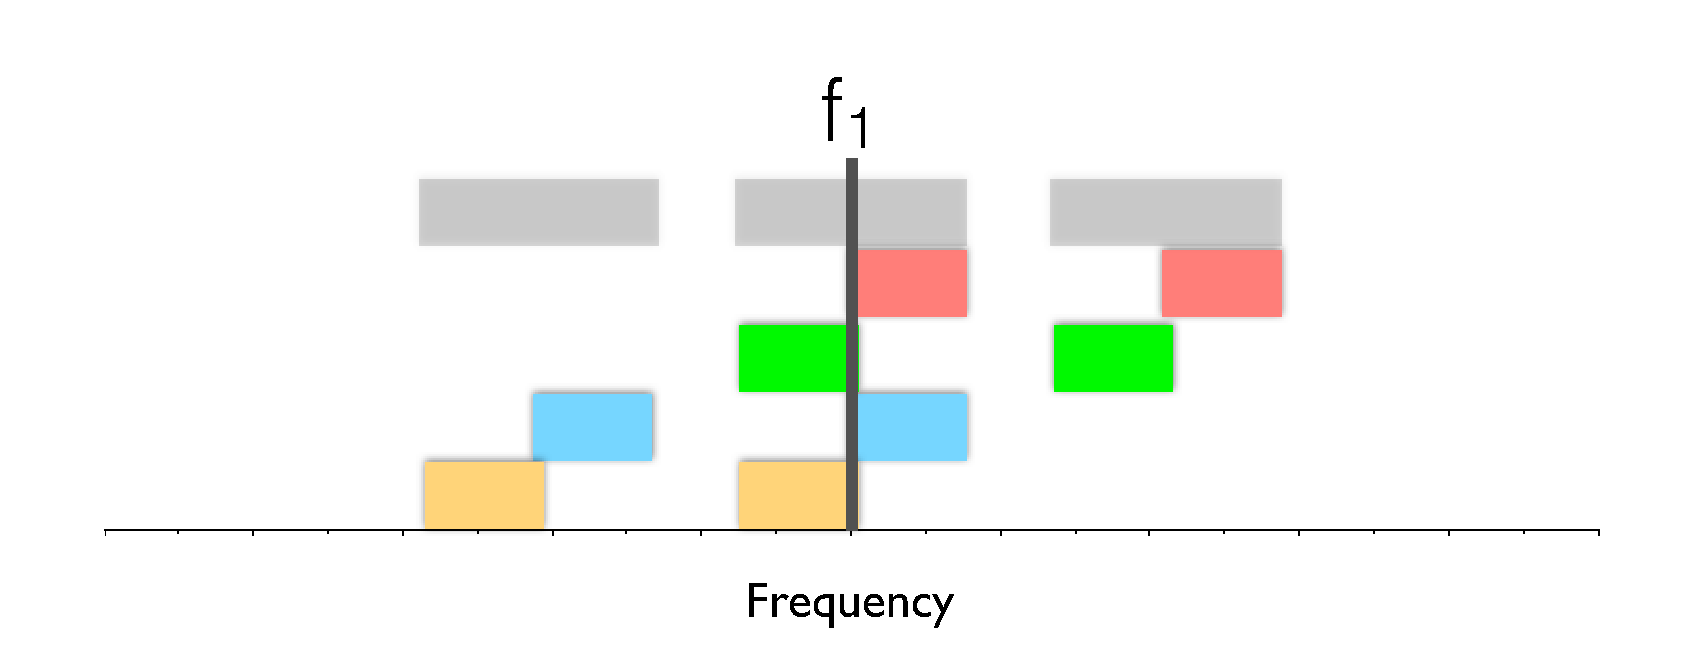
\includegraphics[width=\textwidth]{part10/Williams_O32/O32_f3a.eps}
	\caption{Diagram of how the filter range is derived from the possible tunings for a two-sideband receiver. At the most extreme tunings, the target frequency f$_1$ can be placed in the upper edge (yellow) or lower edge (blue) of the upper sideband, or in the upper edge (green) or lower edge (red) of the lower sideband. The union of these frequency ranges gives the sideband filter for frequency f$_1$ (grey).}
	\label{fig:filter union}
\end{subfigure}%
~~
\begin{subfigure}[b]{0.5\textwidth}
	\centering
	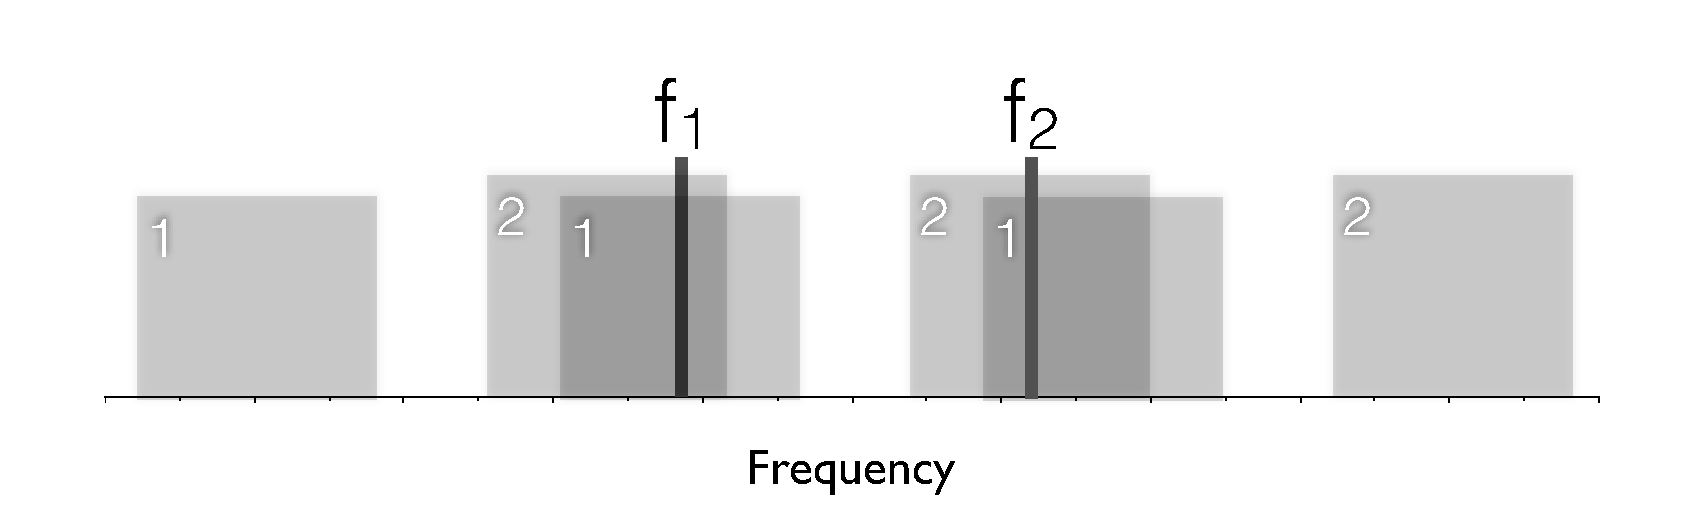
\includegraphics[width=\textwidth]{part10/Williams_O32/O32_f3b.eps}
	\caption{Example of two two-sideband filters combining to restrict the filter window. On selecting frequency f$_1$, sideband filter 1 is created. Frequency f$_2$, lying within filter 1, can be added to the proposal. On addition of f$_2$, sideband filter 2 is added to the filter pipeline. The intersection of these filters, seen as the more opaque region, gives the allowed frequency limits for further line selection.}
	\label{fig:sidebands}
\end{subfigure}%
\caption{Construction and effect of a two-sideband filter on line selection.}
\label{fig:filter construction}
\end{figure}

\acknowledgements The authors would like to thank the Splatalogue team for providing support and the data on which the selector depends, and the ALMA OT testers for consistently driving the case for hardware-aware filtering.

\bibliography{editor}
